%!TEX root = documentation.tex

\chapter*{Acknowledgement}

In first place our special thanks go to Ao.Univ.Prof.Dr. Wolfgang Kastner who had an open ear for our project idea and agreed to be advisor for this project.\\[12pt]

\noindent Furthermore we want to thank Guido Socher from tuxgraphics.org and the customer service team of ThiesKlima for their support.\\[12pt]

\noindent Another person should also be named here is Roman Kreuzhuber who always was on spot with helping hands when we had questions concerning electronics. 

\chapter{Introduction}

\section{Project idea}
The idea to this project came up when I was flying my model helicopter. I was wondering how nasty the wind was these days and that it would have been better not to take off into the skies.

But where should I know the conditions from? The wind speed is always different than the values provided by online weather services.

That was the point I decided to build something on my own, submitting all the weather data to our website so one can decide beforehand whether to drive to our airfield or not.

\section{Available products on the market}
Having a look on the Internet reveals that there are plenty of weather stations available. Nearly all of them provide the basic features like temperature and air pressure measurement and an LCD for presenting the current conditions and/or a small forecast.

Some more expensive devices even provide a wind sensor and can be connected to a computer via USB. The software shipped with these devices also supports uploading of data to a website.

So why spending so much time for creating our own solution? Comparing the specifications of the wind speed sensors for instance shows that these very cheap sensors only have limited quality. Also detecting the wind direction is not available in most products, which is essential for airfield applications.

Another thing is extensibility. We needed a system that can be extended by new sensors easily and that is flexible enough to generate graphs and diagrams as desired.

The result of this investigation is the present project called Flight Weather Station (abbr. FWS).

\section{About FWS} % (fold)
\label{sec:about_fws}

As depicted in Figure~\ref{fig:fws_overview}, FWS consists of the following parts:
\begin{itemize}
\item Sensors: These sensors capture the parameters: Wind speed, wind direction, temperature. Data are transmitted via cable.
\item Slave: The slave collects and processes the data from the sensors.
\item Master: This software collects the processed data of the slave over Ethernet LAN. It generates diagrams and graphs which are sent to the webserver by a separate script.
\item Webserver (Presentation): The generated diagrams are integrated into the website with a plugin for the CMS TYPO3\footnote{\url{http://typo3.org}} also written specifically for this project.
\end{itemize}

The transfer of the data from the master to the webserver isn't part of this project. We recommend using cronjobs or similar approaches to accomplish this task.

\begin{figure}[ht]
    \centering
    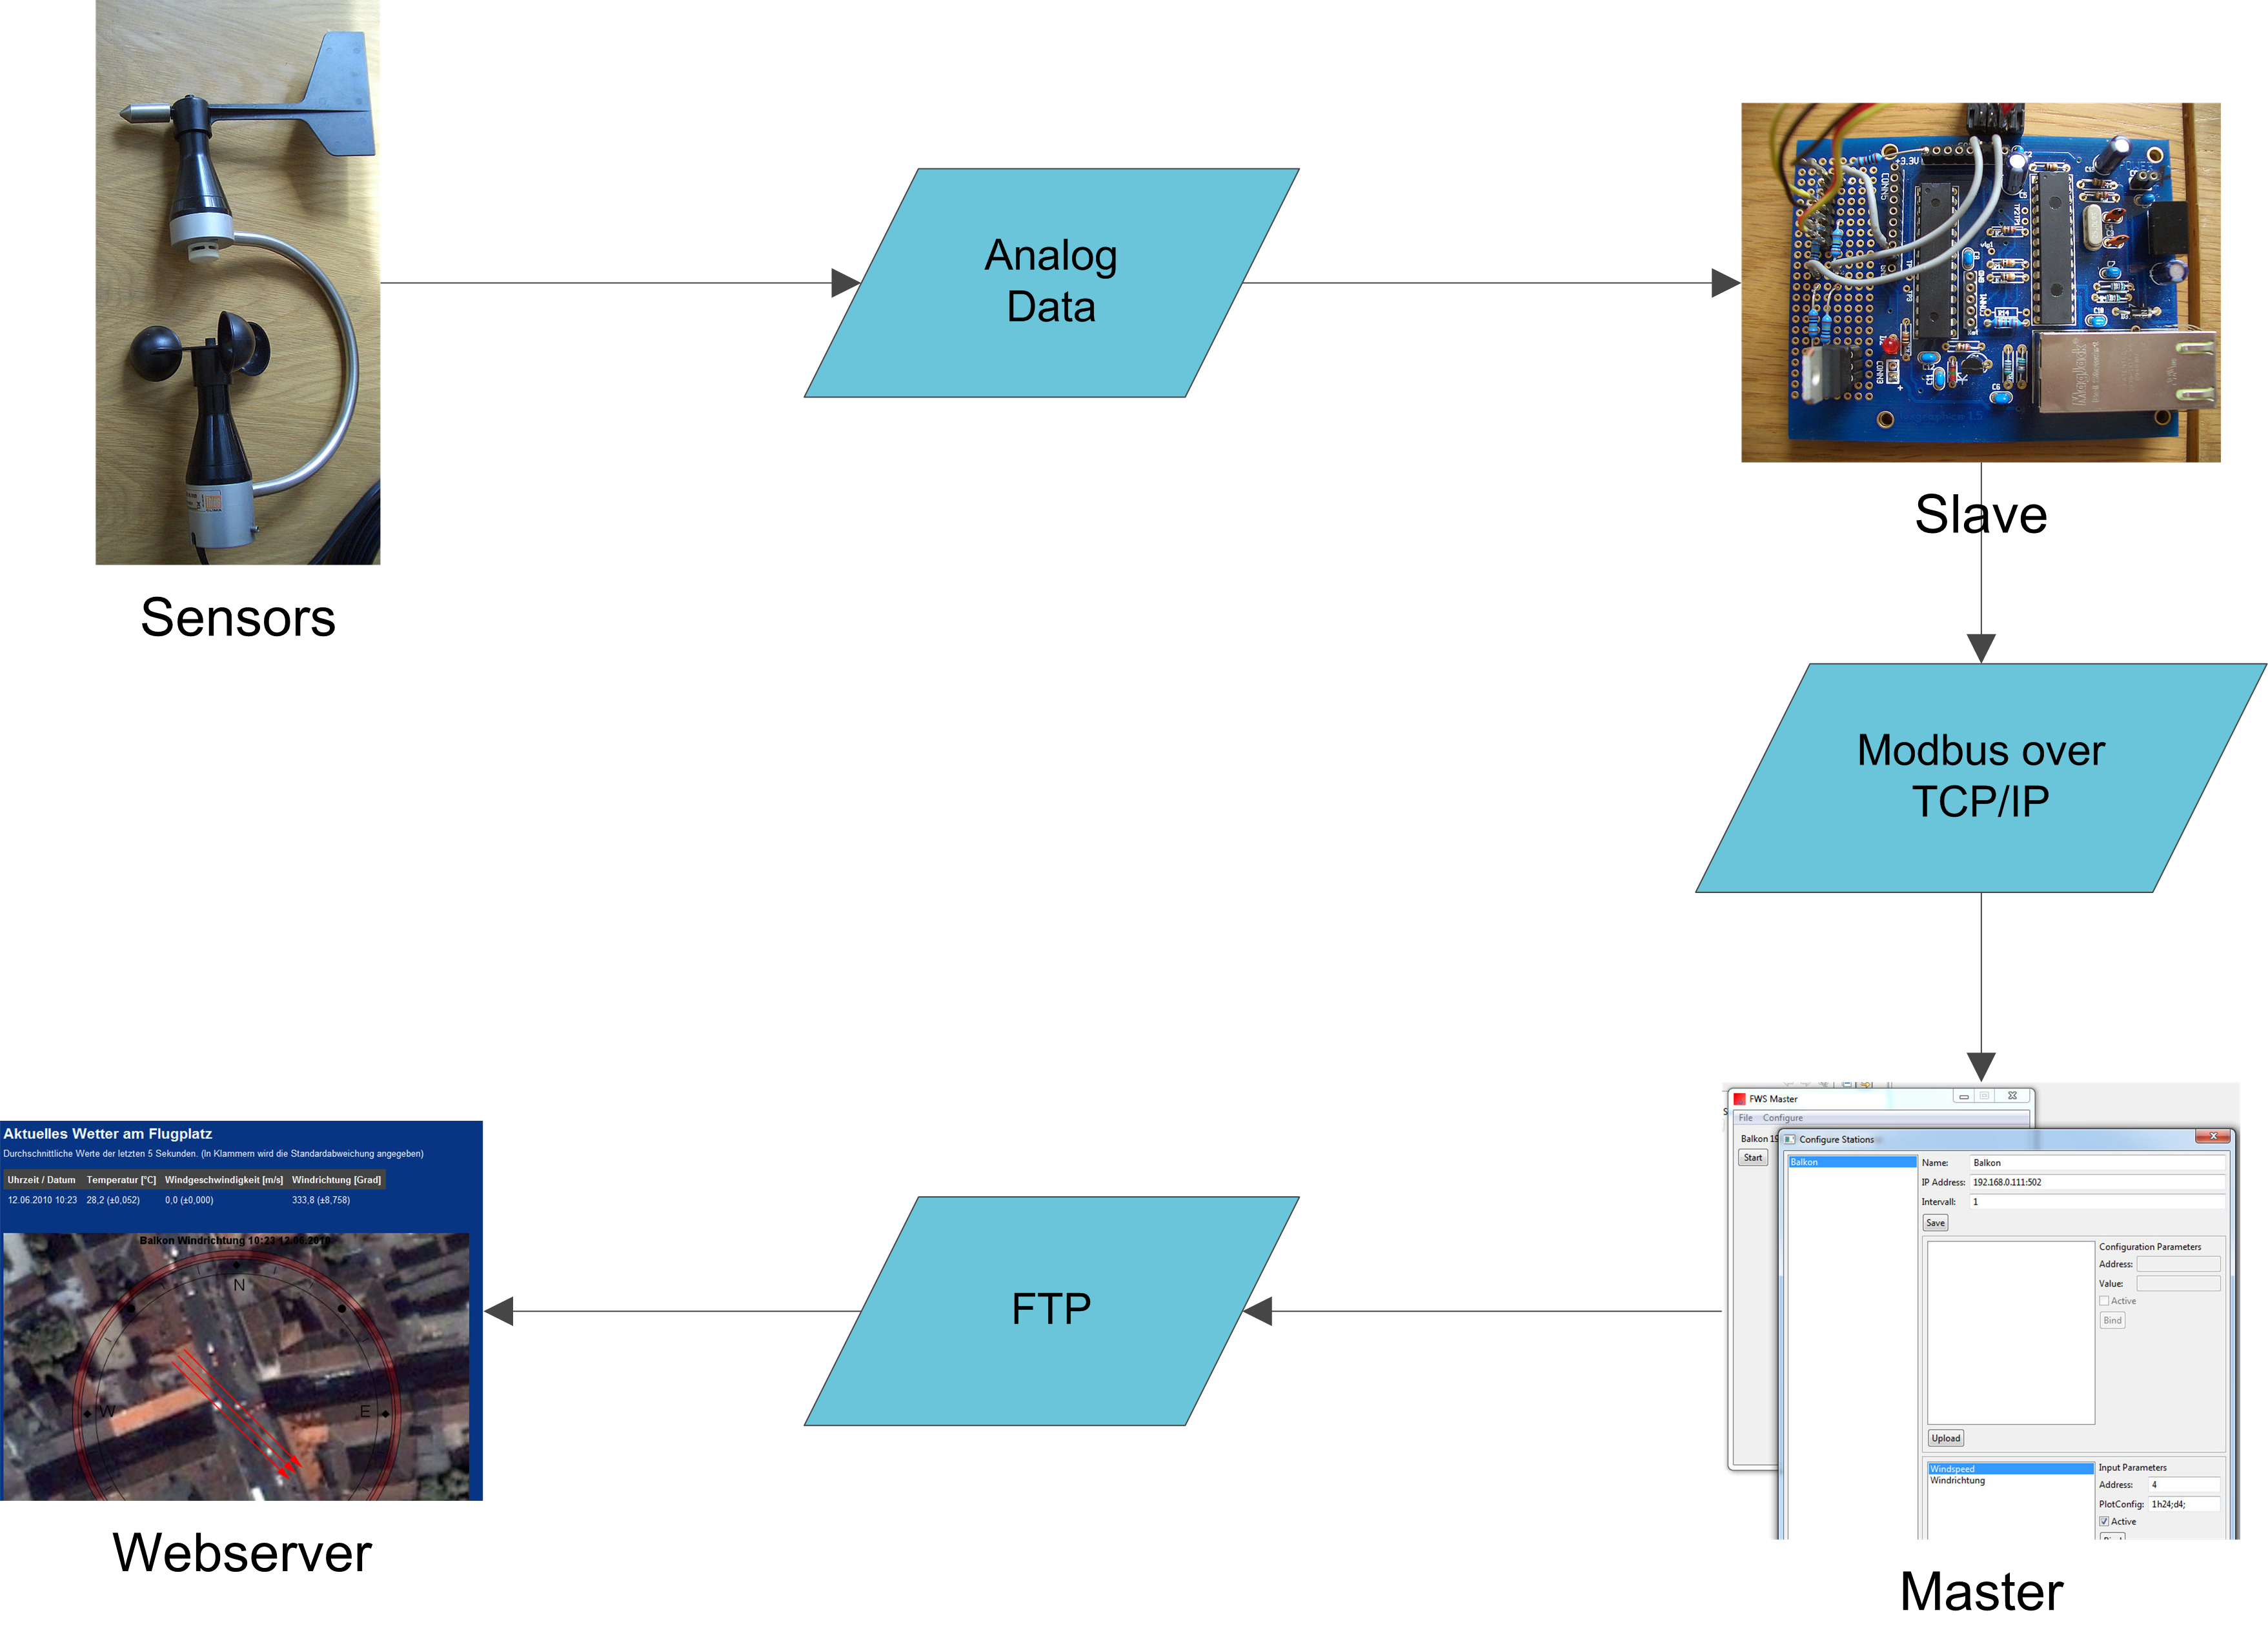
\includegraphics[width=\linewidth]{graphics/overview.png}
    \caption{Module and protocol overview of FWS}
    \label{fig:fws_overview}
\end{figure}

% section about_fws (end)